\section{Task 3: Word Difficulty Classification and Prediction}
\subsection{Weighted Distribution Scoring Model}
To better measure the difficulty of the word by the result distribution of trial times, it is meaningful to assign different weights to different trial times and calculate weighted trial times for 2 reasons:
\begin{itemize}
    \item\textbf{Reason 1: } For most words, most people try 3-5 times to guess, so the trial times between 3-5 usually can't provide valuable information for assessing difficulties.
    
    \item\textbf{Reason 2: } Though relatively few people guess the words for just 1~2 times or more than 6 times, those cases are actually most valuable for assessing difficulties.
\end{itemize}

The goal of \textbf{rating information value and assigning weight} for $t_{i} (i=1,2...,7)$ reminded us of applying \textbf{Entropy Weight Method}. Entropy Weight is found to enhance the function of the attribute with the highest diversity of attribute data (DAD) as well as weaken the function of the attributes with a low DAD in decision-making or evaluation.
\par Since we have n words and 7 indicators to be weighted, we generated the data matrix:
\begin{align}
	X=\left[\begin{array}{cccc}
			t_{11}  & t_{12}  & \cdots & t_{17} \\
			t_{21}  & t_{22}  & \cdots & t_{27} \\
			\vdots  & \vdots  & \ddots & \vdots  \\
			t_{n 1} & t_{n 2} & \cdots & t_{n7}
		\end{array}\right]
\end{align}
\par Then we standardized the data we have and got the standardized matrix $Z=(\tilde{t}_{i j})$,
\begin{align}
	\tilde{t}_{i j}:=\frac{t_{i j}}{\sqrt{\sum\limits_{k=1}^{n} t_{k j}^{2}}}
\end{align}
\par Next, we normalized the data and got the probability matrix $P=(p_{i j})$. 
\begin{align}
	p_{i j}:=\frac{\tilde{t}_{i j}}{\sum\limits_{k=1}^{n} \tilde{t}_{k j}}
\end{align}
\par Finally, we calculated the information entropy and the entropy weight of $t_{i}$ $(i=1,2,...,7)$.
\begin{align}
	e_{j}:=-\frac{1}{\ln n} \cdot \sum_{i=1}^{n} p_{i j} \ln p_{i j}    \quad w_{j}=\frac{1-e_{j}}{\sum\limits_{i=1}^{m} (1-e_{j})}, j=1,2,...,7
\end{align}
\par The \textbf{Weighted Distribution Score} for the $j^{th}$ word is then:
\begin{align}
    s_{i}=\sum_{j=1}^{7}w_{j}\,t_{i\,j}
\end{align}

Generally, a larger weighted distribution score means a greater word difficulty.


%%%%%%%% TODO 计算步骤和可视化美化
\subsection{Word Difficulty Classification Model}

\subsubsection{Difficulty Level Setting}
We set \textbf{4} difficulty Levels for Wordle Game, which were respectively \textbf{Easy, Medium, Hard, Hell} with increasing difficulty. Therefore, the mission is to classify the words given in data set into 4 \textbf{difficulty sets}:

\qquad $U_{1}=\{\text{words} | \text{difficulty = Easy}\}$ \quad $U_{2}=\{\text{words}|\text{difficulty = Medium}\}$

\qquad $U_{3}=\{\text{words} | \text{difficulty = Hard}\}$ \quad $U_{4}=\{\text{words}|\text{difficulty = Hell}\}$

\subsubsection{Indicators for Difficulty Classification}
We select two indicators for difficulty classification:

    (1) \textbf{Trial Time Results Mean ($\mu_{i}$)} \qquad (2) \textbf{Weighted Distribution Score ($s_{i}$)}

Generally, larger $\mu_{i}$ and larger $s_{i}$ indicate higher word difficulty, we believe that considering the distribution of both of them can make our difficulty classification more comprehensive. 

\subsubsection{Word Difficulty Embedding Model}
The words are embedded into $\mathbb{R}^{2}$ vectors. For the $i^{th}$ word, the embedded vector is:
\begin{align}
    x_{i}=(\tilde{\mu_{i}},\tilde{s_{i}})
    \label{z-score}
\end{align}
where $\tilde{\mu_{i}}$ and $\tilde{s_{i}}$ are z-score standardized $\mu_{i}$ and $s_{i}$ 
\subsubsection{Apply Fuzzy C-Means Model (FCM) for Classification}
Since the relationship between words were quite fuzzy, the boundary between each different difficulty modes should be blurred. Therefore, we resorted to \textbf{Fuzzy C-Means Model (FCM)} for word difficulty classification.

First, the centers of four difficulty groups were set to be $c_{i}$, $(i=1,2,3,4)$, and the detailed values were calculated later.

Then, \textbf{Euclidean Distance} was applied for describing the distance between the embedding vectors of words:

\begin{align}
    \mathrm{dist}(c_{i},x_{i})=\|c_{i}-x_{i}\|_{2}
\end{align}



After that, To characterize the fuzziness, we introduced the concept \textbf{membership degree} $u_{i\,j}$,to describe the probability for the $i^{th}$ word to belong to the $j^{th}$ difficulty level:
\begin{align}
    u_{i\,j}=P[word_{i}\in U_{j}]
\end{align}
Since every word must belongs to one difficulty set, we consequently had:
\begin{align}
    \sum_{j=1}^{4}u_{i\,j}=1
\end{align}
Then the \textbf{fuzzy partition matrix} was constructed as $U=(u_{i\,j})$.

Then the target is to minimize the objective function:
\begin{align}
    J(U,C)=\sum_{s=1}^{4}\sum_{i=1}^{n}(u_{is})^{m}\times \mathrm{dist}(c_{i},x_{s})^{2}
    \label{objective-function}
\end{align}
where $m=1.2$ is the arbitrarily-set \textbf{fuzzy exponent} that controls how much the clusters overlap with each other, therefore m describes the fuzziness of difficulty boundaries. 

Then we applied \textbf{Iterative Method} with formulas:
\begin{align}
    u_{i\,j}^{'}=\dfrac{1}{\sum\limits_{k=1}^{4}(\frac{\|x_{i}-c_{j}\|}{\|x_{i}-c_{k}\|})^{\frac{2}{m-1}}}, C_{j}^{'}=\dfrac{\sum\limits_{i=1}^{n}u_{i\,j}^{m}\times x_{i}}{\sum\limits_{i=1}^{n}u_{i\,j}^{m}}
\end{align}
and then the satisfying membership degree matrix $U=(u_{i\,j})$ and centers $C_{i}$ (i=1,2,3,4) were ultimately found to let the objective function (\ref{objective-function}) attain its approximated minimum.

Finally, we classified the words to the difficulty sets to which the words had highest membership degree:
\begin{align}
    \mathrm{level}_{i}=\mathop{\arg\max}_{j} u_{i\,j}
\end{align}

\subsubsection{Accuracy Analysis}
The accuracy for classifying $\mathrm{word}_{i}$,$(i=1,2,...,n)$ can be described by its membership degree $u_{i\,\mathrm{level_{i}}}$.

We calculated the overall accuracy by taking the mean value of accuracy for all the wards in the data set:
\begin{align}
    \mathrm{accuracy}_{cls}=\dfrac{\sum\limits_{i=1}^{n}u_{i\,\mathrm{level_{i}}}}{n}
\end{align}

After examination, we got that $\mathrm{accuracy}_{cls}=96.5\%$, which is really satisfying.
\subsection{Difficulty Classification for Eerie}
With the distribution information acquired in Task 2, the Trial Times Mean and Weighted Distribution Score of "Eerie" can be calculated. We standardized $\mu_{Eerie}$ and $s_{Eerie}$ with the z-score coefficients used in equation (\ref{z-score}) and then we got $\tilde{\mu}_{Eerie}$ and $\tilde{s}_{Eerie}$. Therefore, the embedding $\mathbb{R}^{2}$ vector for "Eerie" is:
\begin{align}
    x_{Eerie}=(\tilde{\mu}_{Eerie},\tilde{s}_{Eerie})
\end{align}

We applied the \textbf{Word Difficulty Classification Model} for "Eerie" and the results were visualized in Figure \ref{cluster}:

\begin{figure}[h]
    \centering
    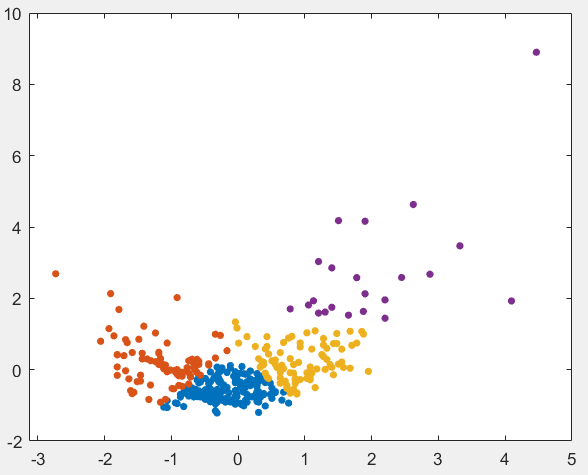
\includegraphics[scale=0.6]{cluster.png}
    \caption{Word Difficulty Classification}
    \label{cluster}
\end{figure}

It can be clearly seen that "Eerie" is classified into the \textbf{Hell Difficulty Category}.
